\documentclass[a4paper]{article}

\usepackage[T2A]{fontenc}
\usepackage[utf8]{inputenc}
\usepackage{textcomp}
\usepackage{amsmath, amssymb}
\usepackage{mathtext}
\usepackage[russian]{babel}
\usepackage{mathtools}
\usepackage{mathtext}
\usepackage{verbatim}
%\usepackage{bm}
\usepackage{enumitem}
%\usepackage{showframe}

\usepackage[paperwidth=205mm, paperheight=260mm, top=2cm, bottom=2cm, left=2cm, right=2.5cm]{geometry}
% figure support
\usepackage{import}
\usepackage{xifthen}
\pdfminorversion=7
\usepackage{pdfpages}
\usepackage{transparent}
\newcommand{\incfig}[1]{%
    \def\svgwidth{\columnwidth}
    \import{./figures/}{#1.pdf_tex}
}
\usepackage{indentfirst}
\pdfsuppresswarningpagegroup=1
\usepackage{amsthm}
\theoremstyle{plain}
\newtheorem*{thm}{Theorem}
\newtheorem{lem}[thm]{Lemma}
\newtheorem{prop}[thm]{Proposition}
\newtheorem*{cor}{Corollary}

\theoremstyle{definition*}
\newtheorem*{defn}{Definition}
\newtheorem{conj}{Conjecture}[section]
\newtheorem*{exmp}{Example}

\theoremstyle{remark}
\newtheorem*{rem}{Remark}
\newtheorem*{note}{Note}

\newcommand{\defeq}{\vcentcolon=}
\newcommand{\eqdef}{=\vcentcolon}
\newcommand{\rpm}{\raisebox{.2ex}{$\scriptstyle\pm$}}

\usepackage{listings}
\usepackage{graphicx}
\lstset{
  frame=tb,
  language=C++,
  extendedchars=\true,
  inputencoding=utf8,
  keepspaces = true, 
  aboveskip=3mm,
  belowskip=3mm,
  showstringspaces=false,
  columns=flexible,
  basicstyle={\small\ttfamily},
  numbers=left,
  numberstyle=\tiny\color{gray},
  keywordstyle=\color{blue},
  commentstyle=\color{dkgreen},
  breaklines=true,
  breakatwhitespace=true,
  tabsize=3
}
\usepackage{hyperref}
\usepackage{float}
\begin{document}

\begin{titlepage}
\begin{center}
\Large{МИНОБРНАУКИ РОССИИ}

\large{ФЕДЕРАЛЬНОЕ ГОСУДАРСТВЕННОЕ АВТОНОМНОЕ ОБРАЗОВАТЕЛЬНОЕ УЧРЕЖДЕНИЕ \\
ВЫСШЕГО ОБРАЗОВАНИЯ}

\large{\bfseries САНКТ-ПЕТЕРБУРГСКИЙ \\
ПОЛИТЕХНИЧЕСКИЙ УНИВЕРСИТЕТ ПЕТРА ВЕЛИКОГО}

\vspace{1.05 cm} 
Институт прикладной математики и механики

\vspace{1.05 cm} 
Высшая школа прикладной математики и вычислительной физики
\end{center}

\vspace{1cm}

\begin{center}
{ 
\large    Отчёт по дисциплине:\\
	``Дискретная математика''\\
    \textbf{Лабораторная работа № 2} \\
     Реализация булевых функций

}
\end{center}

\vspace{5cm}


\begin{center}
	\begin{tabular}{cccc}
		{\normalsize Выполнил:} & \underline{\hspace{3cm}} & {\normalsize студент группы 3630201/90001} &{\normalsize Волынец А.В.} \\
		{\normalsize	Принял:} & \underline{\hspace{3cm}} & {\normalsize Востров A.В.} \\
	\end{tabular}
\end{center}

\vspace{1.8cm}
\begin{center}
Санкт-Петербург — 2020
\end{center}

\end{titlepage}

\tableofcontents 
\newpage

\section*{Введение}
\addcontentsline{toc}{section}{Введение}


В данной лабораторной работе требуется по таблице истинности булевой 
функции построить сокращенное дерево решений и наиболее компактную 
бинарную диаграмму решений, а также синтаксическое дерево и 
логическую схему на основе дизъюнктора, конъюктора и инвертора. Реализовать
программно вычисление значений булевой функции через бинарную диаграмму 
решений. Программно с помощью таблицы истинности построить СДНФ и СКНФ. 
Вычислить программно по СДНФ значения булевой функции. Вычисление 
значений функции по СДНФ и БДР (бинарной диаграмме решений) должны
совпадать с таблицей истинности. Также для данной функции необходимо
программно построить полином Жегалкина. 


Исходная функция, заданная с помощью вектора значений по возрастанию аргументов: 
\[
    f(x, y, z, k) = (0000010110011111)
\] 

\newpage
\section{Математическое описание задачи}
\subsection{Вычисление СДНФ и СКНФ по таблице истинности}
\begin{defn}
    Совершенной дизъюнктивной нормальной формой (СДНФ) булевой функции 
    $\displaystyle f(x_1, \ldots, x_{n})$ называется формула $\displaystyle F$
    в базисе Буля вида: 
     \[
         F: f(x_1, \ldots, x_{n}) = 
         \underset{\{(\left \sigma_1, \ldots, \sigma_{n} \right)| 
     f(\sigma_1, \ldots, \sigma_{n}) = 1\}}{\bigvee} x^{\sigma_{1}}_{1} \ldots
     x_{n}^{\sigma_{n}}
    \] 
\end{defn}
\begin{defn}
    Совершенной конъюктивной нормальной формой (СКНФ) булевой функции 
    $\displaystyle f(x_1, \ldots, x_{n})$ называется формула $\displaystyle G$
    в базисе Буля вида: 
     \[
         G: f(x_1, \ldots, x_{n}) = 
         \underset{\{(\left \sigma_1, \ldots, \sigma_{n} \right)| 
     f(\sigma_1, \ldots, \sigma_{n}) = 0\}}{\bigwedge} x^{\overline{\sigma_{1}}}_{1} \vee \ldots
 \vee x_{n}^{\overline{ \sigma_{n}}}
    \] 
\end{defn}


С помощью таблицы истинности всегода можно найти СДНФ и СКНФ по 
определению. Для функции $\displaystyle f$:

\[
       f(x, y, z, k) = (0000010110011111)
\] 


СДНФ($\displaystyle f$) =  $\displaystyle \overline{x}y\overline{z}k  
\vee \overline{x}yzk \vee x\overline{y} \overline{z} \overline{k}
\vee x\overline{y} zk \vee xy\overline{z}\overline{k} \vee 
xy\overline{z}k \vee xyz\overline{k} \vee xyzk$


СКНФ($\displaystyle f$) = $\displaystyle \left( x \vee 
y \vee z \vee k  \right)
\left( x \vee y \vee x \vee \overline{k}  \right)
\left( x \vee y \vee \overline{z}  \vee k  \right)
\left( x \vee y \vee \overline{z}  \vee \overline{k}  \right) 
\left( x \vee \overline{y}  \vee z \vee k  \right) 
\left( x \vee \overline{y}  \vee \overline{z} \vee k  \right) $
$\left( \overline{x}  \vee y \vee z \vee \overline{k} \right) 
\left( \overline{x}  \vee y \vee \overline{z}  \vee k  \right) $


\subsection{Построение полинома Жегалкина}
\begin{defn}
    Полиномом Жегалкина булевой функции $\displaystyle f(x_1, \ldots, x_{n})$ 
    называется формула $\displaystyle F$ в базисе Жегалкина 
    $\displaystyle \left( \wedge, + \right) $:
    \[
        F: f(x_1, \ldots, x_{n}) =  \alpha_0 + \alpha_1x_1 + \alpha_2x_2 +
        \ldots + \alpha_{123\ldots n}x_1\ldots x_{n}
    \] 
\end{defn}


Для функции $\displaystyle f$ полином Жегалкина имеет вид: 
\[
    f(x, y, z, k) = \alpha_0 + \alpha_1 k + \alpha _2 z + 
    \alpha_3 zk + \alpha_4 y + \alpha_{5}yk + \ldots + \alpha_{15} xyzk
\]  
Построение методом треугольника: 
\vspace{-0.3 cm}
\begin{flalign*}
    \alpha_0 &=  0000010110011111 \\
    \alpha_1 &=   000011101010000\\
 \alpha_2  &=  00010011111000\\
 \alpha_3 &= 0011010000100\\
 \alpha_4 &=     010111000110\\
 \alpha_5 &=     11100100101\\
 \alpha_6 &=     0010110111\\
 \alpha_7  &=  011101100\\
 \alpha_8   &= 10011010\\
 \alpha_9 &=     1010111\\
 \alpha_{10} &=     111100\\
 \alpha_{11} &=    00010\\
 \alpha_{12} &=   0011\\
 \alpha_{13} &=    010\\
   \alpha_{14} &=   11\\
    \alpha_{15} &=  0\\
\end{flalign*}
Откуда следует, что полином Жегалкина: 
\[
    f(x, y, z, k) = yk + x + xk + xz + xyz
\] 
\subsection{Дерево решений}
Для данной функции построено сокращенное дерево решений, которое 
получается из бинарного дерева решений заменой узлов дающих одно 
значение этим значением: 

\begin{figure}[H]
    \centering
    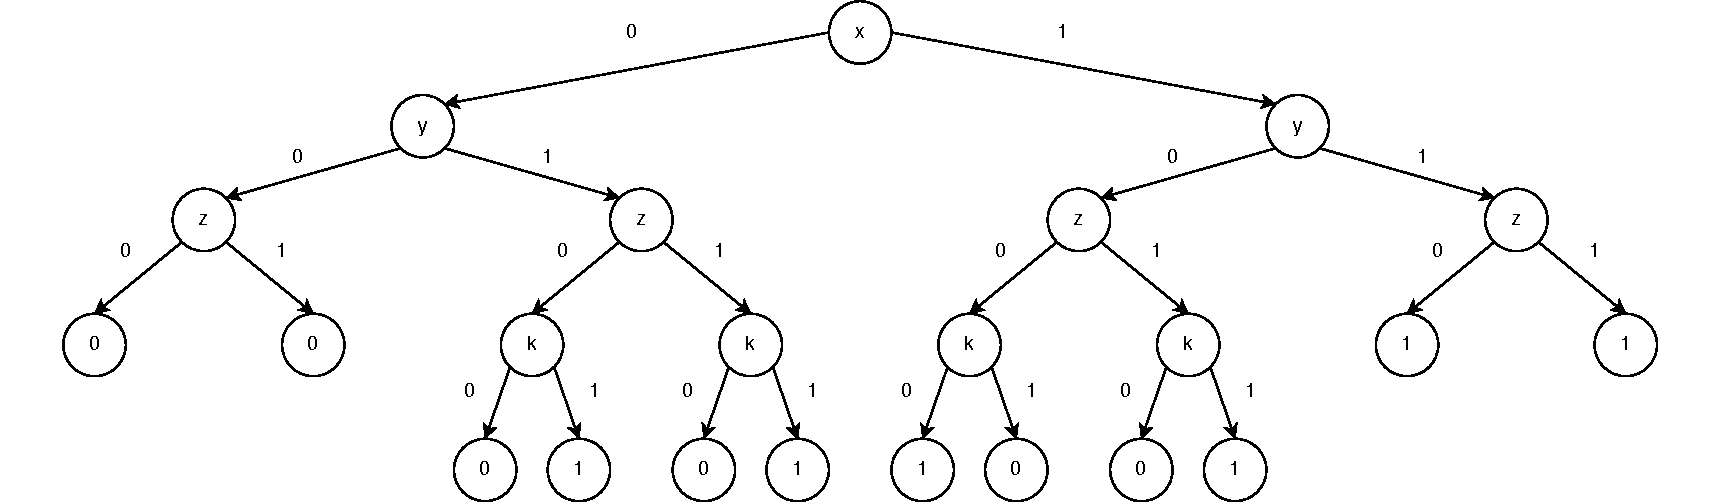
\includegraphics[width=0.8\textwidth]{pics/ShortTree.pdf}
    \caption{Сокращенное дерево решений}
\end{figure}

\subsection{Бинарная диаграмма решений}
Бинарная диаграмма решений получается из дерева решений допущением
вхождения нескольких дуг в один узел. Для функции $\displaystyle f$ 
построена бинарная диаграмма решений:

\vspace{1 cm}
\begin{figure}[H]
    \centering
    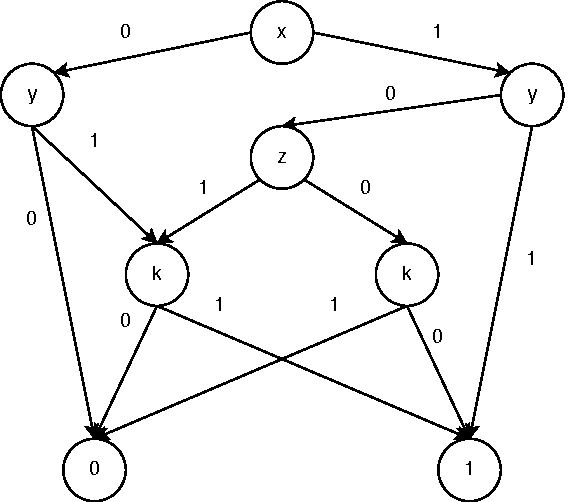
\includegraphics[]{pics/BDR-2.pdf}
    \caption{Бинарная диаграмма решений}
    \label{fig:}
\end{figure}

\newpage
\subsection{Синтаксическое дерево}
Для минимальной формы функции $\displaystyle f = xy \vee yk \vee xyk \vee x
\overline{z} \overline{k} $
построено синтаксическое дерево: 

\vspace{1 cm}
\vspace{1 cm}
\begin{figure}[H]
    \centering
    \input{SyntacsTree-2.pdf_tex}
    \caption{Синтаксическое дерево для минимальной формы}
    \label{fig:}
\end{figure}

\newpage
\subsection{Логическая схема}
Для минимальной формы функции $\displaystyle f = xy \vee yk \vee xyk \vee x
\overline{z} \overline{k} $
построена логическая схема на основе дизъюнктора, конъюктора и
инвертора (рис. 4): 

\vspace{2 cm}
\begin{figure}[H]
    \centering
    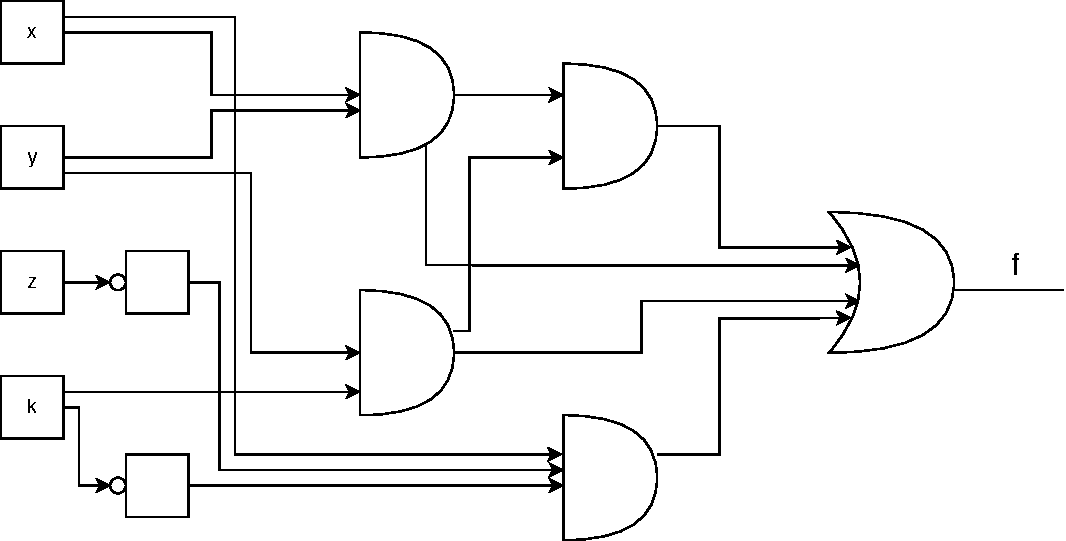
\includegraphics[width=0.8\textwidth]{pics/Log-2.pdf}
    \caption{Логическая схема}
\end{figure}

\newpage
\section{Особенности реализации}

Для хранения данных используются глобальные переменные, поэтому многие 
функции не имеют параметров. Булева функция $\displaystyle f$ 
задаётся с помощью \lstinline{vector<char>}:
\begin{lstlisting}
vector<char> func{0, 0, 0, 0, 0, 1, 0, 1, 1, 0, 0, 1, 1, 1, 1, 1};
\end{lstlisting}
\subsection{Программное построение СДНФ и СКНФ}
Для построения СДНФ по таблице истинности используется следующий 
алгоритм 3.3 ([1], стр. 135): 
\begin{figure}[htpb]
    \centering
    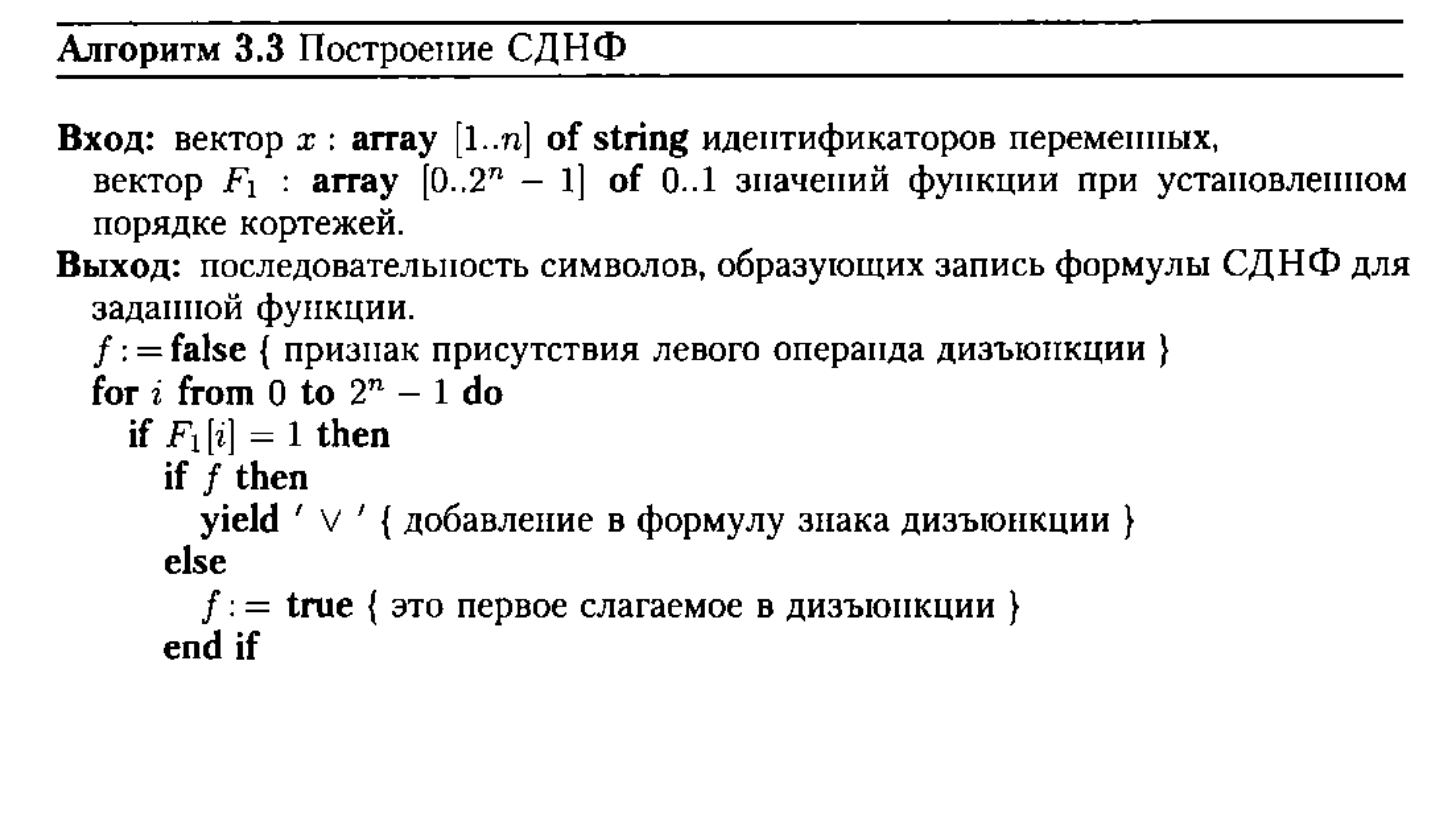
\includegraphics[width=0.8\textwidth]{pics/SDNF1}
\end{figure}
\vspace{-2.3 cm}

\begin{figure}[htpb]
    \centering
    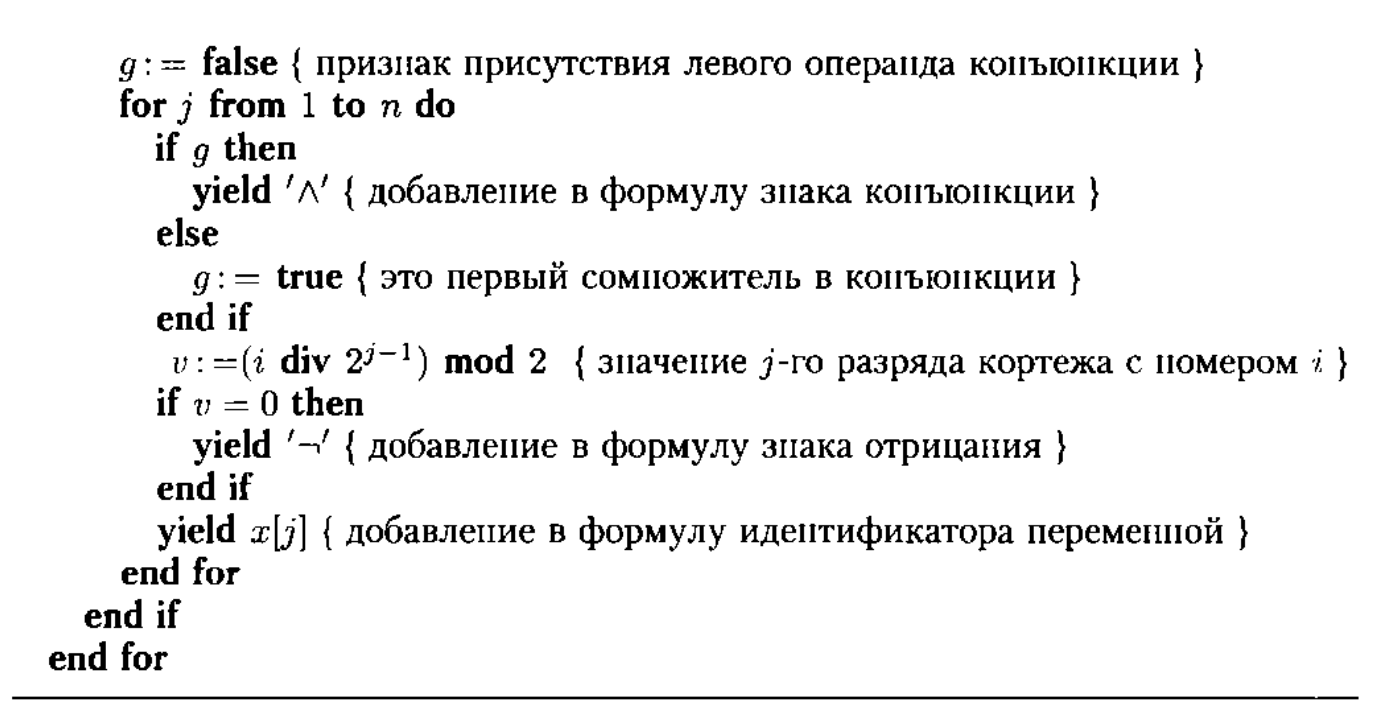
\includegraphics[width=0.8\textwidth]{pics/SDNF2}
\end{figure}

В программе массиву индентификаторов соответствует: 
\begin{lstlisting}
const char* ids = "xyzk";
\end{lstlisting}

Результат алгоритма сохраняется в переменной sdnf типа \lstinline{string}.
Построение СКНФ происходит по аналогичному алгоритму. 
\newpage
\subsection{Вычисление значения функции по СДНФ}
Вход: строковое представление СДНФ, аргумент булевой функции типа int


Выход: bool - значение функции при данном аргументе. 


При первом вызове функции инициализируется статический двумерный массив 
\lstinline{vector<vector<char> table}, в котором хранятся кортежи, 
при которых функция принимает значение $\displaystyle 1$.
\begin{lstlisting}
bool calcOnSDNF(int i){
    static size_t count = 0;
    static vector<vector<char>> table;
    if (count == 0){
        int term = -1;
        for (int k = 0; k < sdnf.size(); k++) {
            if (sdnf[k] == 'x') {
                table.emplace_back();
                if (k > 0 and sdnf[k - 1] == '!')
                    table[++term].push_back(0);
                else
                    table[++term].push_back(1);
            }
            else if (sdnf[k] == 'y' or sdnf[k] == 'z' or sdnf[k] == 'k'){
                if (k > 0 and sdnf[k - 1] == '!')
                    table[term].push_back(0);
                else
                    table[term].push_back(1);
            }
        }
        count++;
    }
    ...
\end{lstlisting}

Далее значение аргумента \lstinline{i} переводится в двоичную систему 
счисления в массив \lstinline{vector<char> value}. После чего 
данный кортеж сравнивается с кортежами в массиве table:
\begin{lstlisting}
...
    vector<char> value(toBin(i));
    bool res = true;
    for (int k = 0; k < table.size(); k++){
        res = true;
        for (int j = 0; j < len; j++){
            if (table[k][j] != value[j]){
                res = false;
                break;
            }
        }
        if (res) return true;
    }
    return res;
}
\end{lstlisting}

\newpage
\subsection{Вычисление значения функции по БДР}
Бинарная диаграмма решений реализована в виде класса 
\lstinline{BinaryDiagram} и вспомогательного класса вершины
\lstinline{Node}:
\begin{lstlisting}
struct Node{
    Node* l_child; //указатель на узел по нулевому ребру 
    Node* r_child; //указатель на узел по единичному ребру
    bool val;
    Node(): l_child(nullptr), r_child(nullptr), val(false){}
    Node(Node* l, Node* r, bool v = false): l_child(l), r_child(r), val(v){}
};

struct BinaryDiagram{
    const int N = 9;// число вершин графа
    std::vector<Node*> nodes;
    ...
}
\end{lstlisting}

В конструкторе класса устанавливаются потомки узлов БДР через 
вспомогательный метод SetChildren. БДР, использующееся в программе 
отличается от привиденного на рис. 2. Для реализации алгоритма вычисления
значения по БДР нужно добавить фиктивные узлы между внутренними узлами,
если путь (количество ребер) меньше чем количество переменных. Так 
было добавлен узел с номером 8 между узлами 1 и 4, как показано 
на рис. 4. Номерам узлов соответствуют индексы массива nodes. 

\begin{figure}[htpb]
    \centering
    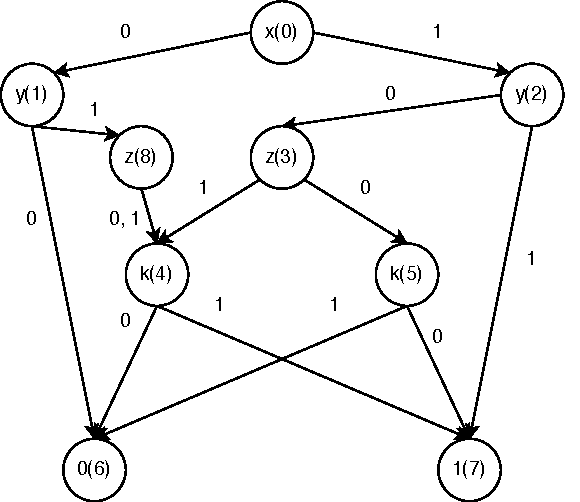
\includegraphics[scale = 0.7]{pics/BDR-3.pdf}
    \caption{Внутренее представление БДР}
    \label{fig:BDR-3-pdf}
\end{figure}

Ниже приведен конструктор класса Binary Diagram:


Вход: нет параметров


Выход: нет возвращаемого значения, иниацилизируется массив 
nodes, задающий БДР
\begin{lstlisting}
    BinaryDiagram(): root(nullptr), nodes(N, nullptr){
        for (int i = 0; i < N; i++){
            nodes[i] = new Node;
        }
        setChildren(0, 1, 2);
        setChildren(1, 6, 8);
        setChildren(8, 4, 4);
        setChildren(2, 3, 7);
        setChildren(3, 5, 4);
        setChildren(4, 6, 7);
        setChildren(5, 7, 6);
        nodes[6]->val = false;
        nodes[7]->val = true;
    }
\end{lstlisting}
Ниже приведен вспомогательный для конструктора метод setChildren:


Вход: i - номер родителя, l - номер левого ребенка, r - номер правого
ребёнка. 


Выход: нет возвращаемого значения, метод устанавливает поля 
l\_child и r\_child структуры node с номером i в массиве nodes.

\begin{lstlisting}[]
    void setChildren(int i, int l, int r){
        nodes[i]->l_child = nodes[l];
        nodes[i]->r_child = nodes[r];
    }
\end{lstlisting}


Вычисление значения 
функции реализовано с помощью следующей процедуры: 


Вход: корень БДР Node*, аргумент типа int, для которого нужно вычислить 
значение функции. 


Выход: значение функции при данном аргументе - bool
\begin{lstlisting}
bool BinaryDiagram::calc(int i){
    vector<char> value(toBin(i));
    Node* p = nodes[0];
    for (int k = 0; k < value.size(); k++){
        if (p->r_child == nullptr and p->l_child == nullptr)
            return p->val;
        else if (value[k] == 0)
            p = p->l_child;
        else
            p = p->r_child;
    }
    return p->val;
}
\end{lstlisting}
Метод calc проходит по дереву решений, пока не дойдет до вершины 
самого нижнего яруса, в которой хранится значение функции при данном
аргументе. 

\subsection{Построение полинома Жегалкина}
Вход: массив значений булевой функции func \lstinline{vector<char>}


Выход: строковое представление полинома Жегалкина jegal
\begin{lstlisting}[]
void findJEGAL()
{
    vector<char> triangle(func.size(), 0);
    for (int i = 0; i < triangle.size(); i++)
        triangle[i] = func[i] - '0';
    bool f = false;
    for (int i = 0; i < (int)pow(2, len); i++)
    {
        if (i != 0) 
        {
            for (int j = 0; j < (int) pow(2, len) - i; j++) 
            {
                triangle[j] ^= triangle[j + 1];
            }
        }
        if (triangle[0] == 1)
        {
            if (f)
                jegal += " + ";
            else
                f = true;
            vector<char> value(toBin(i));
            if (i == 0) jegal += "1";
            else{
                for (int k = 0; k < len; k++) {
                    if (value[k]) jegal += ids[k];
                }
            }
        }
    }
} 
\end{lstlisting}

Данная функция строит полином Жегалкина по методу треугольника. 

\newpage
\section{Результаты работы программы}
Ниже приведены результаты работы программы: 
\begin{figure}[htpb]
    \centering
    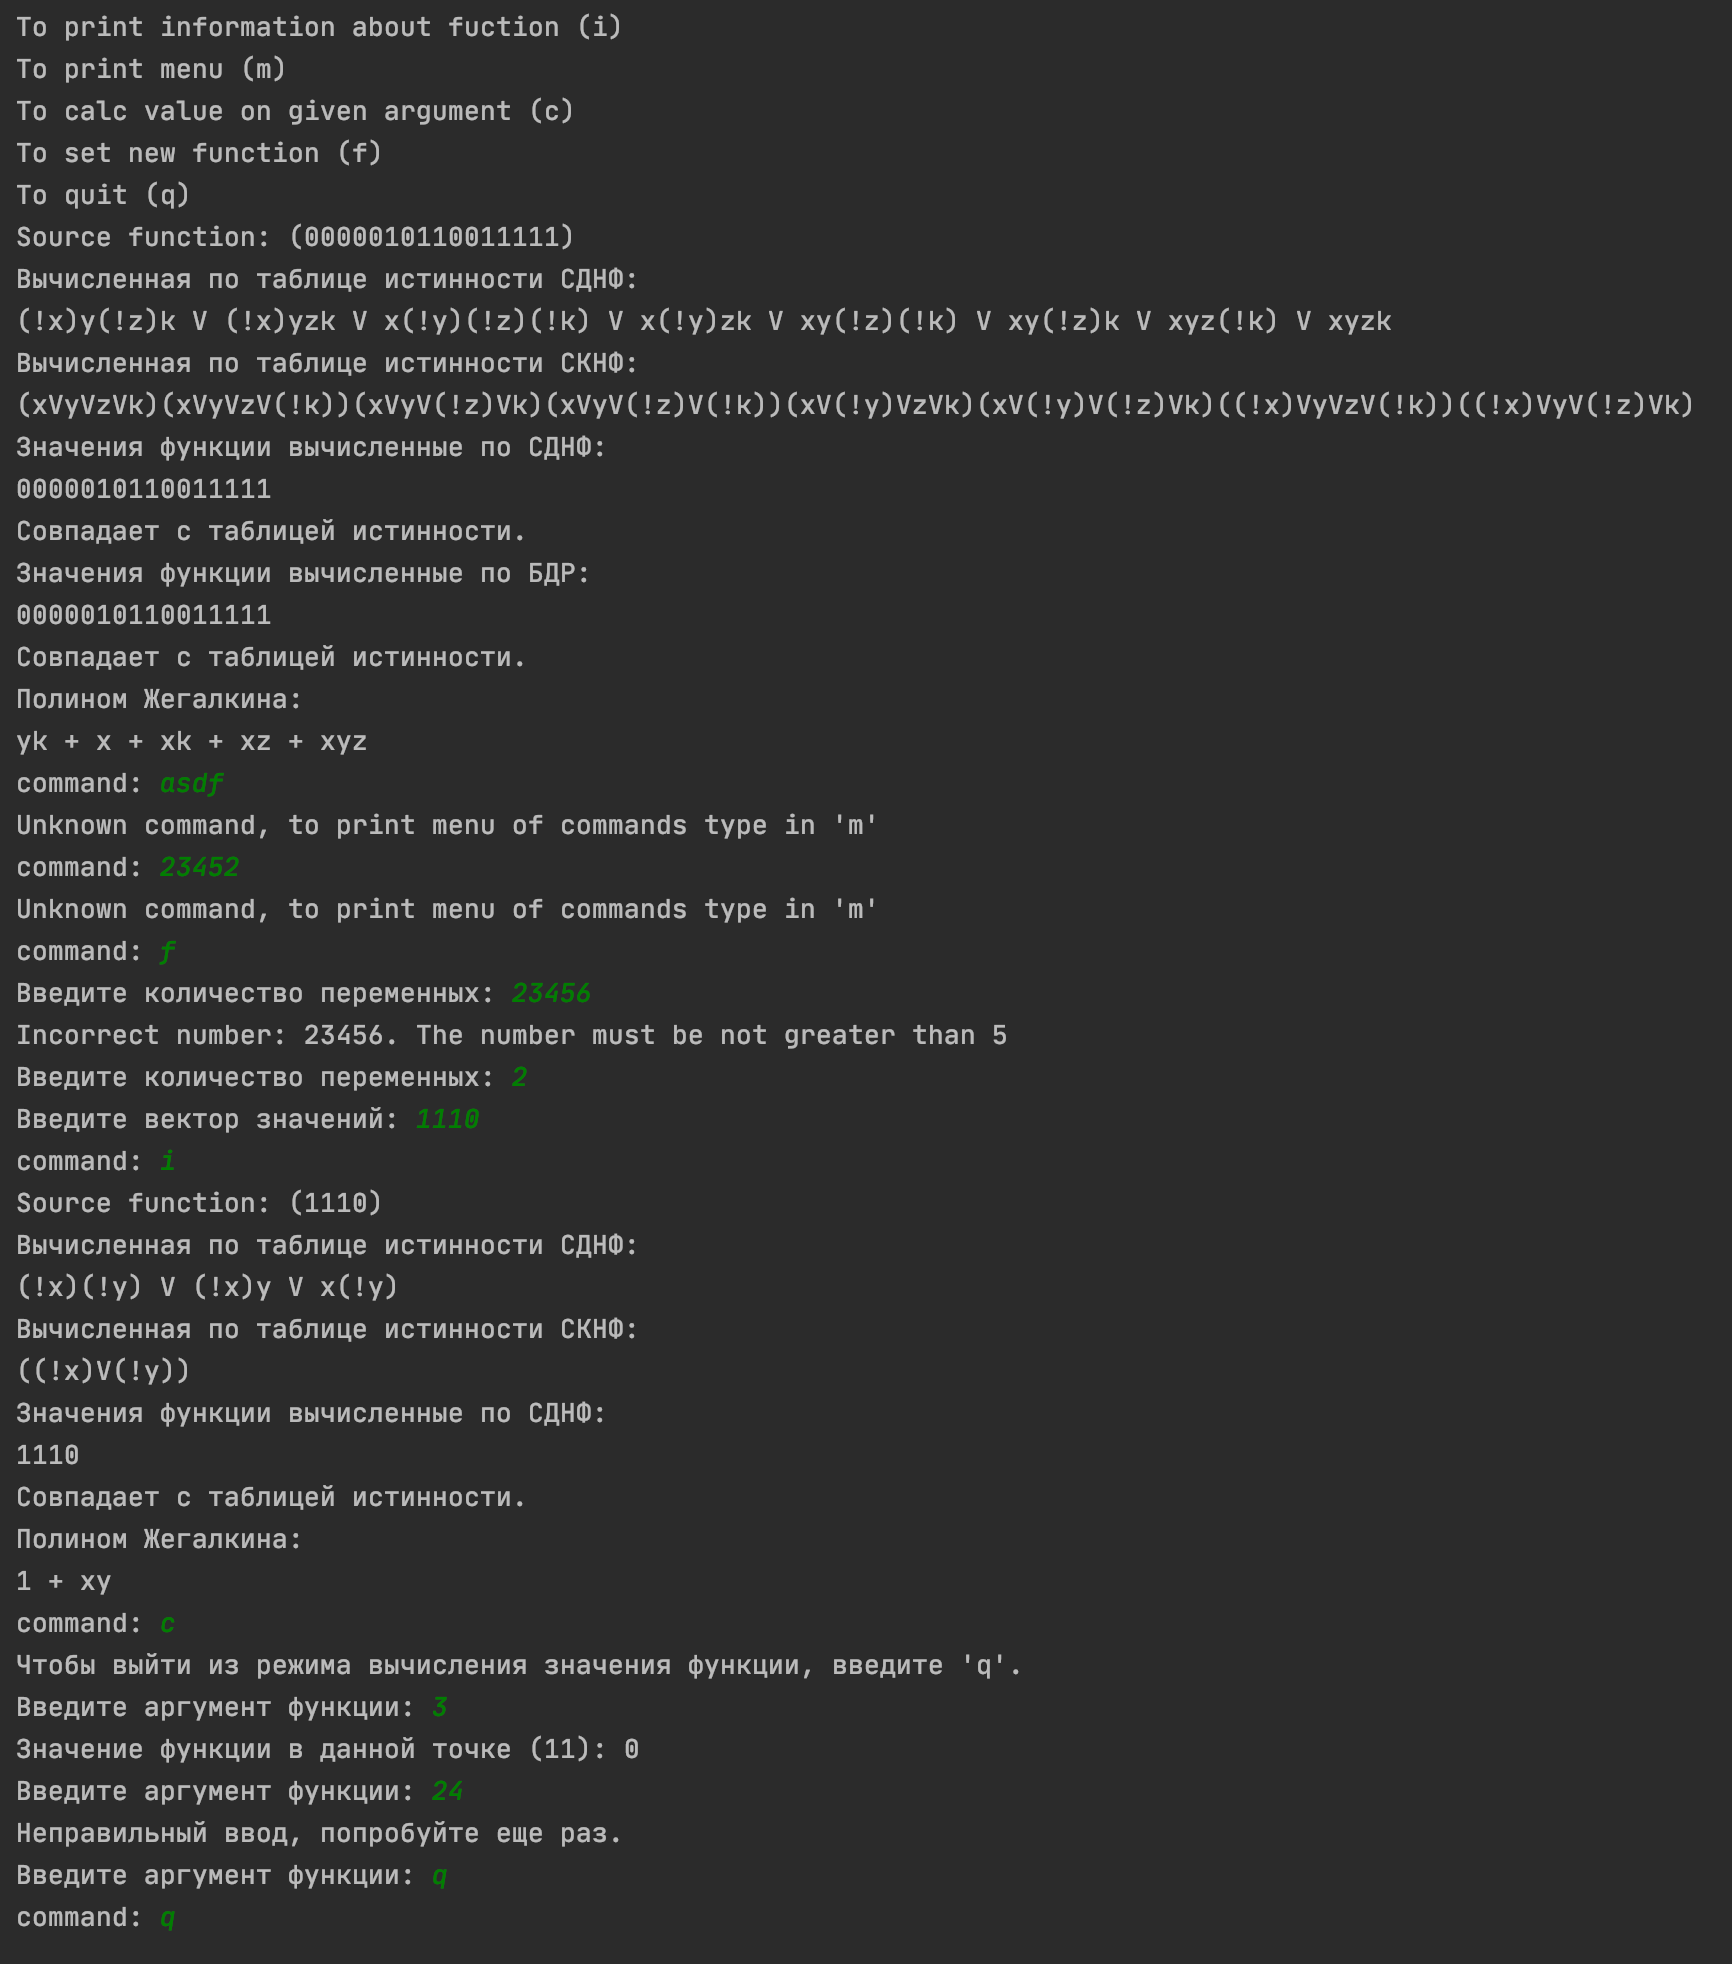
\includegraphics[width=0.8\textwidth]{pics/work}
    \caption{Пример работы программы}
    \label{fig:work}
\end{figure}

На рис. 6 приведена работа программы: сначала выводятся информация
о исходной фукнции из задания, затем пользователь задаёт новую 
функцию двух переменных. Также приведена обработка ошибочного 
пользовательского ввода. 

\newpage
\section*{Заключение}
\addcontentsline{toc}{section}{Заключение}
В данной лабораторной работе для заданной функции $\displaystyle f$ были 
построены сокращенное дерево 
решений, синтаксическое дерево решений, а также бинарная диаграмма
решений. Были построены программно СДНФ, СКНФ, полином Жегалкина для
$\displaystyle f$. 
Были реализованы функции для вычисления значения булевой функции 
через СДНФ и БДР. 


Достоинства программы: 
\begin{enumerate}
    \item Масшатабируемость: возможность программно добавлять
        новые функции с большим количеством переменных и другими
        обозначениями переменных; возможность программно добавлять
        новые функции для работы с булевыми функциями, например 
        минимизации функции. 
    \item Пользовательский интерфейс, который можно модифицировать
        программно при добавлении новых возможностей программы.
    \item Возможность пользователя задавать функцию с меньшим или 
        большим количеством переменных непосредственно при работе
        с программой
    \item Реализована защита от неправильного пользовательского ввода. 
\end{enumerate}


Недостатки программы:
\begin{enumerate}
    \item Бинарная диаграмма решений строится вручную и задаётся в 
        конструкторе класса вручную, при использовании других 
        функций пользователю необходимо программно задать
        БДР.
\end{enumerate}
\newpage
\section*{Список литературы}
\addcontentsline{toc}{section}{Список литературы}
[1] Новиков Ф.А. Дискретная математика для программистов. Учебник для вузов.
3-е изд. - СПб.:Питер, 2001, 304.

[2] Stroustrup B. The C++ programming language, 4-th edition - Addison-Wesley, 2013, 1347. 
\end{document}
